%% Intended to be included into a larger document
\chapter{Related Works}

%% Add more to introduce topics in this chapter?

\section{Why Games}
\label{sec:why-games}

Gamification is not about games, in fact as a subject gamification is deals with everything else but games. But the research in gamification have to largely base on the studies of games. The games already prove to be an effective engaging media and ubiquitous as every day life. In fact, "video game is everywhere" is the critical thesis of many gamification advocates. 

[need more data on game market, player demography]

The following sections will examine a few most popular games and genre to understand what game mechanics give games such power nowaday.

\subsection{Casual Game: Angry Birds}
In today's tech world, no gaming platform is completed without the new star game Angry Birds. There  are over 50 million individuals have downloaded this simple game. The total number of hours consumed by world-wide players is roughly 200 million minutes a day, that is 1.2 billion hours a year.  According to Neiman Journalism Lab[ref], all person-hours spent creating and updating the entire wikipedia totals about 100 million hours.  That is half day of the Angry Birds play time. Why is this seemly simple game so massively compelling? Charles Mauro [ref] discussed the cognitive teardown of Angry Birds in Human factor engineering (aka usability engineering) for the sake of answering the more "important" real world question, "why users don't find their company's software or product engaging?":
    * Simple Engaging Interaction Concept:  Angry Birds' simple interaction model is easy to learn and incremental increase of complexity.
    * Cleverly managed response time: In Angry Birds design, it is not "faster is better", instead, different birds have different trajectory time and the flight path of the bird is intentionally illustrated. It solved one huge problem for user interfaces - error correction.It also take a seemly long time for the pigs to expire once their hours are collapsed, this non-functional time delay increases the playfulness of the game and bring users entertainment.

\subsection{Social Game: Zynga-Ville}
With the motto  "Connecting the world through games", Zynga who found in 2007 quickly become the top game company catching up to the more traditional establishment such as EA and Activision Blizzard. With the help of socal network platform Facebook, the FarmVille and CityVille quickly become the most popular games within Facebook. Zynga later expanded the games into other platform such as mobile and  new google+ social network. 
[more research on Zynga's game number, total time played, total player, compared to Angry Birds]
One distinct characteristic of Zynga games is that they are social and they are all interconnect through an exchangable virtual currency "Zynga Points". 
[more on virtual currency's social effect]

\subsection{MMORPG: World of Warcraft}
[insert the statistics here for comparision with the above, time, player]

\section{Game Mechanics}
There are many game mechanics make game a game. 

\subsection{Status}
This include experience points(XP), ranks on the leader board, health.

\subsection{Achievement}
This normally represents as badge, completed quests.

\subsection{Level progression}

\subsection{Mission Quest Journey}

\subsection{Social}

\subsection{Virtual good or Real-world tangibles reward}

\subsection{Immediate feedback}

\section{Gamification Debates}

\subsection{Can you gamify a suicide hotline?}
Can you gamify everything? "No, you can not gamify game". According to Gabe Zichermann, the idea of baking game mechanics into everything you do is fun, but when asked how would you make a suicide hotline fun, he admitted that adding games to a suicide prevention seems distasteful at first, but he could add a game mechanics like a competitive environment in a call center setting.

\subsection{Gamification is bull*it}

\subsection{Gamification vs Serious game}
Serious game are generally defined[ref], �to include games that make use of computer technology and advanced video graphics and that are used for the purposes of learning and training.�

\section{How to use game mechanics in gamification}

\subsection{Gamification Applications}

\subsection{Smart Gamification}

\section{Gamification Service or Platform}
This section outlines the current industry players that provides gamifcation service via platforms or consultation service. [see figure 2.1]

\begin{figure}[ht]
	\centering
		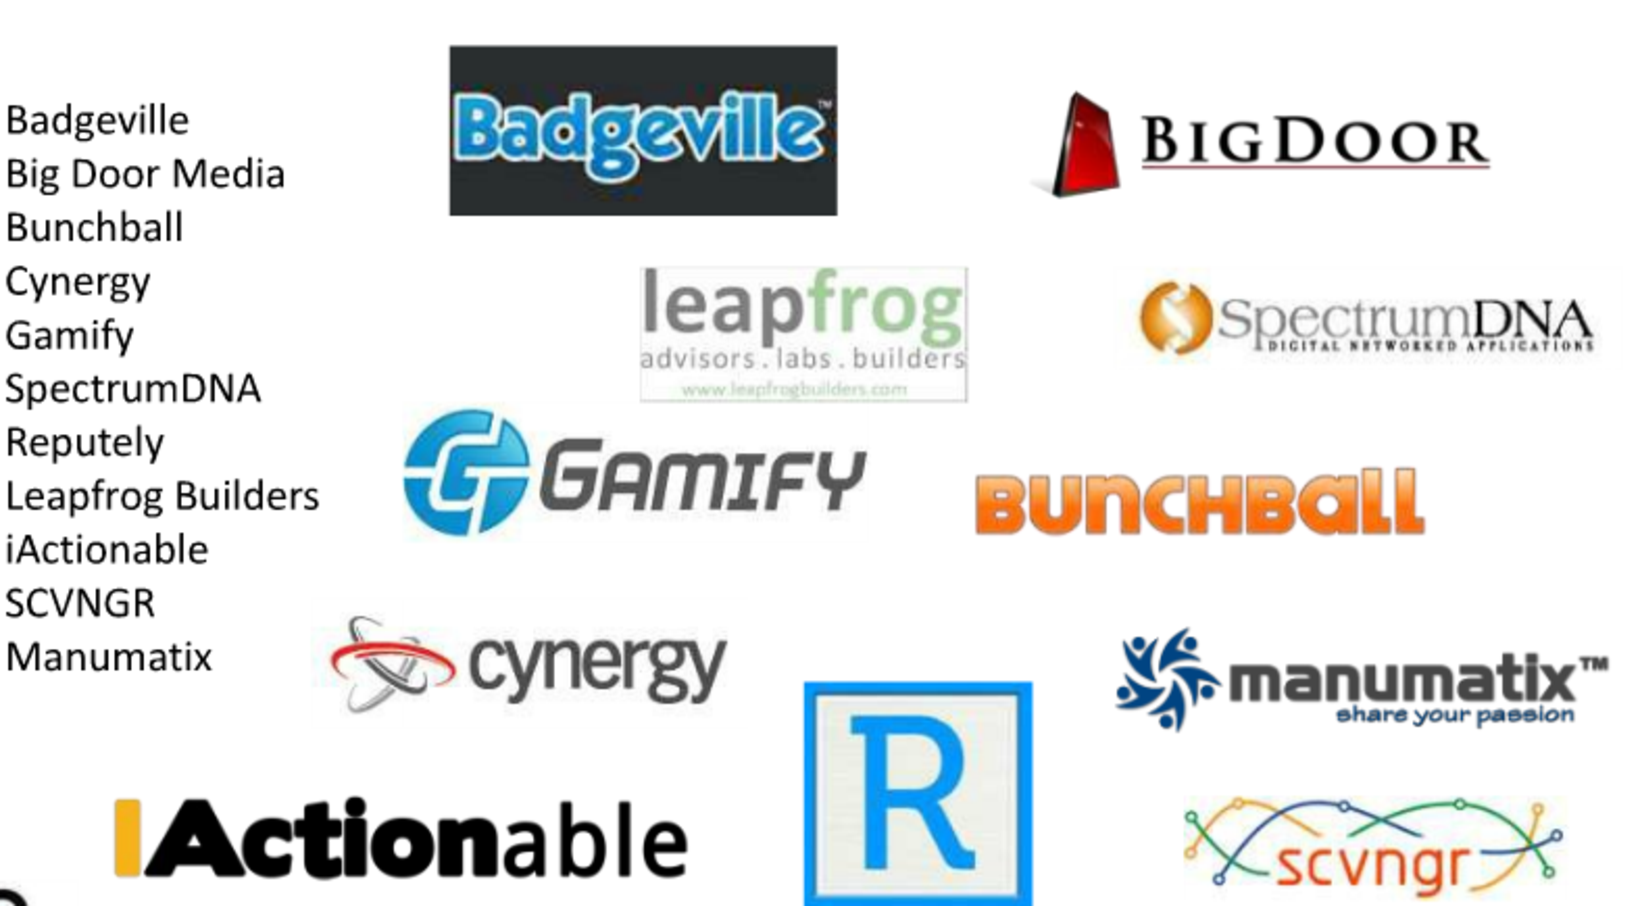
\includegraphics[scale=0.59]{gamification-service.pdf}
		\caption{Gamification Service Industry}
		\label{fig:gamification-service}
\end{figure}


\subsection{Gamification Analytics}
The objective evaluation of Player Experience (PX)[ref] in games is the goal of game metrics and analytics research. With the technology advancement, it is possible to automatically log numerical informations on in-game player behaviour and analyze them in different context. This methodology provides a qualitative and quantitative result of the player experience in games, which in turn affect the result of gamification.



